\documentclass{article}\usepackage[]{graphicx}\usepackage[]{color}
%% maxwidth is the original width if it is less than linewidth
%% otherwise use linewidth (to make sure the graphics do not exceed the margin)
\makeatletter
\def\maxwidth{ %
  \ifdim\Gin@nat@width>\linewidth
    \linewidth
  \else
    \Gin@nat@width
  \fi
}
\makeatother

\definecolor{fgcolor}{rgb}{0.345, 0.345, 0.345}
\newcommand{\hlnum}[1]{\textcolor[rgb]{0.686,0.059,0.569}{#1}}%
\newcommand{\hlstr}[1]{\textcolor[rgb]{0.192,0.494,0.8}{#1}}%
\newcommand{\hlcom}[1]{\textcolor[rgb]{0.678,0.584,0.686}{\textit{#1}}}%
\newcommand{\hlopt}[1]{\textcolor[rgb]{0,0,0}{#1}}%
\newcommand{\hlstd}[1]{\textcolor[rgb]{0.345,0.345,0.345}{#1}}%
\newcommand{\hlkwa}[1]{\textcolor[rgb]{0.161,0.373,0.58}{\textbf{#1}}}%
\newcommand{\hlkwb}[1]{\textcolor[rgb]{0.69,0.353,0.396}{#1}}%
\newcommand{\hlkwc}[1]{\textcolor[rgb]{0.333,0.667,0.333}{#1}}%
\newcommand{\hlkwd}[1]{\textcolor[rgb]{0.737,0.353,0.396}{\textbf{#1}}}%

\usepackage{framed}
\makeatletter
\newenvironment{kframe}{%
 \def\at@end@of@kframe{}%
 \ifinner\ifhmode%
  \def\at@end@of@kframe{\end{minipage}}%
  \begin{minipage}{\columnwidth}%
 \fi\fi%
 \def\FrameCommand##1{\hskip\@totalleftmargin \hskip-\fboxsep
 \colorbox{shadecolor}{##1}\hskip-\fboxsep
     % There is no \\@totalrightmargin, so:
     \hskip-\linewidth \hskip-\@totalleftmargin \hskip\columnwidth}%
 \MakeFramed {\advance\hsize-\width
   \@totalleftmargin\z@ \linewidth\hsize
   \@setminipage}}%
 {\par\unskip\endMakeFramed%
 \at@end@of@kframe}
\makeatother

\definecolor{shadecolor}{rgb}{.97, .97, .97}
\definecolor{messagecolor}{rgb}{0, 0, 0}
\definecolor{warningcolor}{rgb}{1, 0, 1}
\definecolor{errorcolor}{rgb}{1, 0, 0}
\newenvironment{knitrout}{}{} % an empty environment to be redefined in TeX

\usepackage{alltt}
\usepackage[sc]{mathpazo}
\usepackage[T1]{fontenc}
\usepackage{geometry}
\geometry{verbose,tmargin=2.5cm,bmargin=2.5cm,lmargin=2.5cm,rmargin=2.5cm}
\setcounter{secnumdepth}{2}
\setcounter{tocdepth}{2}
\usepackage{url}
\usepackage[unicode=true,pdfusetitle,
            bookmarks=true,bookmarksnumbered=true,bookmarksopen=true,bookmarksopenlevel=2,
            breaklinks=false,pdfborder={0 0 1},backref=false,colorlinks=false]
{hyperref}
\hypersetup{
  pdfstartview={XYZ null null 1}}
\usepackage{breakurl}
\IfFileExists{upquote.sty}{\usepackage{upquote}}{}
\begin{document}




\title{STAT 585X - Final Project - Draft Report \\ Changes in cultivated cropland soil in Iowa }

\author{Andreea Erciulescu}
\maketitle


\section{Introduction}

\subsection{Question of interest}


Do soil characteristics changes over time match the Conservation Effects Assessement Project (CEAP) survey design and data collection?

\subsection{Motivation}

National Resources Inventory (NRI) is an annual survey conducted collaboratively by USDA NRCS (Natural Resources Conservation Services) and ISU Center for Survey Statistics and Methodology (CSSM) to provide status and trend estimates for natural resources on nonfederal lands in US. Example of such estimates are soil erosion estimates in relation to land characteristics and programs.\\

Conservation Effects Assessment Project (CEAP) is a series of surveys intended to quantify environmental effects of conservation prctices and programs by hydrologic unit codes (HUCs). The following image illustrates the division of the United States territory into 2-digits HUCs and the sudivision of the Upper Mississippi region into 4-digit HUCs.  

\begin{center}
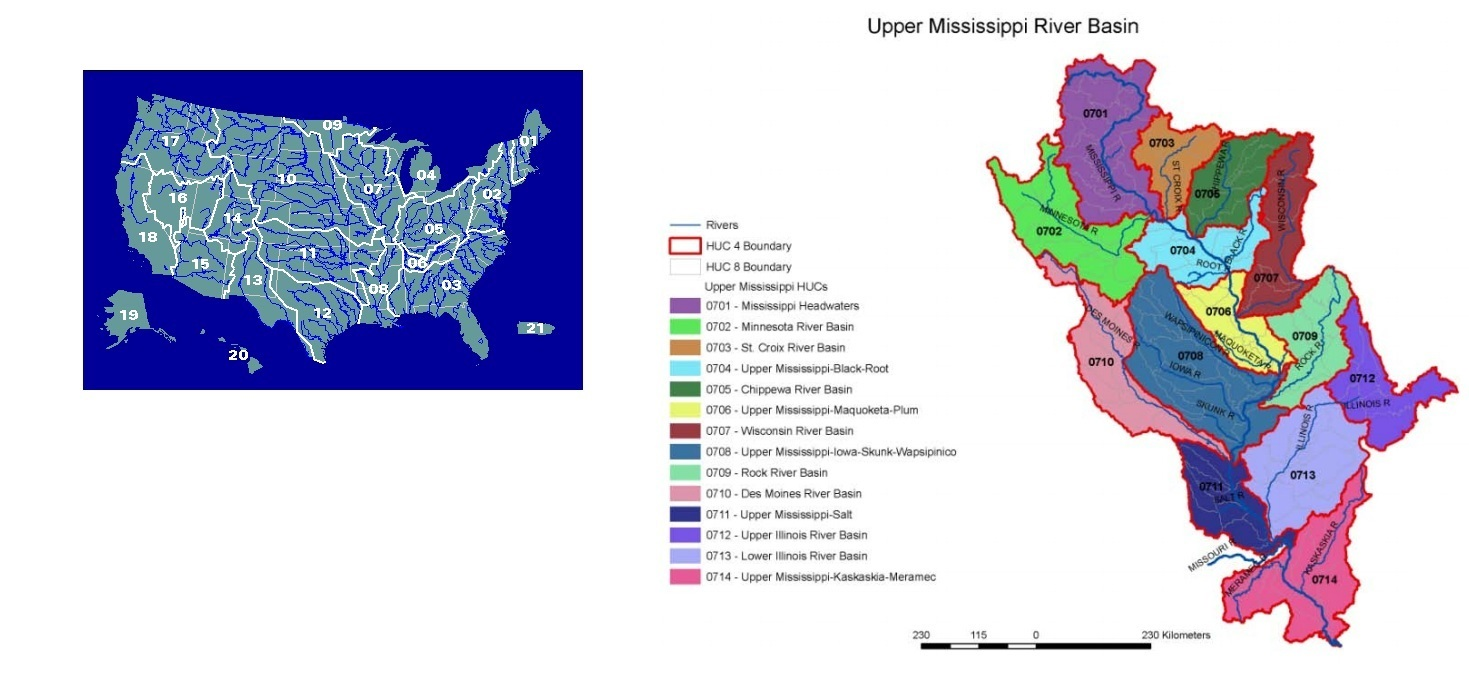
\includegraphics[width=16cm, height=8cm]{HUC2-4-8.jpg} 
\end{center}

The CEAP sample is a subset of the NRI points classified as cultivated cropland. The data was collected using farmers interviews and NRCS hydrologic, climate and soil databases. The data was then filtered through an APEX model (black box) and the result is a set of observations for usable points for 19 response variables. The final goal is to produce erosion estimates for 8-digit HUCs. \\

CEAP is run at both national and regional levels. Among the regional levels, the Des Moines River Watershed (HUC 0710) is a region of interest in this project, that is subdivided into 9 8-digit HUCs.\\

For analysis, data from the Soil Survey is considered, collected over the 2003 to 2006 time period. Hence, the survey frame, consisting of NRI cultivated cropland points, is set in 2003. The information for these eligible points is collected in the following years, 2004-2007.


\subsection{Data}

The CEAP sample data for the Des Moines River Watershed (HUC 0710) region is not publicly available, so in the class project I will consider the following sources of information:

\begin{itemize}

\item Crop Data Layer (CDL)\\


The CDL data is available at \href {CDL} {http://nassgeodata.gmu.edu/CropScape/} in the form of Tagged Image File (.tif) Format. We are interested in the state of Iowa data, available for the years of 2003-2007. The information consists of pixel counts and acreage values for different category of cropland data. Each of the category has an associated value (code), for example 1 stands for Corn and 5 stands for Soybean. A complete list of category codes, class names and colors for the USDA NASS CDL is available at \href{Codes}{http://www.nass.usda.gov/research/Cropland/docs/CDL_2013_crosswalk.htm}.


\item Census Topologically Integrated Geographic Encoding and Referencing database (Tigerweb) \\


The Census Tigerweb data is available at \href{Census}{http://tigerweb.geo.census.gov/tigerwebmain} for both national and regional leveles. Also, data for the hydrologic levels is available at 

\href{HydroCensus}{http://tigerweb.geo.census.gov/tigerwebmain/Files/tigerweb_tab10_hydro_poly_ia.html}. We are interested in the state of Iowa data, as well as the Des Moines River data. In particular, we are interested in the points coordinates. 


\item Public Land Survey System (PLSS)\\

The PLSS data can be found on \href{PLSS}{http://http://www.geocommunicator.gov/GeoComm/lsis_home/home/index.htm} in the form of shapefiles. Information is available at both state and county levels.  
\item   GIS data on hydrologic basins\\

The GIS data can be found at \href{GIS}{ftp://ftp.igsb.uiowa.edu/gis_library/basins/} in the form of shapefiles. Information is available for the entire Des Moines River basin.

\item   Atlas of historical countyu boundaries (AtlasHCB)\\

The AtlasHCB data is available at \href{AtlasHCB}{http://publications.newberry.org/ahcbp/pages/Iowa.html} in the form of shapefiles. Information os available for the entire state of Iowa.

\section{Data Collection and Processing Steps}

We are going to explore all these different data sources and decide on the most useful one. We are interested in a very specific region in the state of Iowa so we would have to be careful at utilizing the data. Also, the files have very large dimensions, so we would have to be careful at selecting the amount of useful information.

\subsection{CDL data}

We first download the data for years 2003-2007 from the website \href {CDL} {http://nassgeodata.gmu.edu/CropScape/}. We have five .tif files, one for each year of interest. These are raster graphics images, spatial data structures that divide the US teritory into pixels that store crop information. This type of data are referred to as a 'grid,' contrasted with 'vector' data is used to represent points, lines, polygons. The dimensions of files are very large \footnote{After saving the data to my U drive I received an e-mail from the university alerting me that I have filled $99\%$ of my Cyfiles. Hence, I opened a Cybox account and started to move other folders over.}.\\

An useful R package to read and manipulate these data is the \textit{Raster} package. This package allows us to read the raster values from the files and to convert the cell numbers to coordinates and back. \\

\begin{knitrout}
\definecolor{shadecolor}{rgb}{0.969, 0.969, 0.969}\color{fgcolor}\begin{kframe}
\begin{alltt}
\hlkwd{setwd}\hlstd{(}\hlstr{"U:/classes/585X"}\hlstd{)}
\hlkwd{library}\hlstd{(}\hlstr{"raster"}\hlstd{)}
\end{alltt}


{\ttfamily\noindent\itshape\color{messagecolor}{\#\# Loading required package: sp}}\begin{alltt}
\hlcom{# ?raster ####S4 methd}

\hlcom{## read the data}
\hlstd{cdl.ia03} \hlkwb{<-} \hlkwd{raster}\hlstd{(}\hlstr{"data/cdl/CDL_2003_19.tif"}\hlstd{)}
\end{alltt}


{\ttfamily\noindent\itshape\color{messagecolor}{\#\# rgdal: version: 0.8-14, (SVN revision 496)\\\#\# Geospatial Data Abstraction Library extensions to R successfully loaded\\\#\# Loaded GDAL runtime: GDAL 1.10.1, released 2013/08/26\\\#\# Path to GDAL shared files: C:/Program Files/R/R-3.0.2/library/rgdal/gdal\\\#\# GDAL does not use iconv for recoding strings.\\\#\# Loaded PROJ.4 runtime: Rel. 4.8.0, 6 March 2012, [PJ\_VERSION: 480]\\\#\# Path to PROJ.4 shared files: C:/Program Files/R/R-3.0.2/library/rgdal/proj}}\begin{alltt}
\hlstd{cdl.ia04} \hlkwb{<-} \hlkwd{raster}\hlstd{(}\hlstr{"data/cdl/CDL_2004_19.tif"}\hlstd{)}
\hlstd{cdl.ia05} \hlkwb{<-} \hlkwd{raster}\hlstd{(}\hlstr{"data/cdl/CDL_2005_19.tif"}\hlstd{)}
\hlstd{cdl.ia06} \hlkwb{<-} \hlkwd{raster}\hlstd{(}\hlstr{"data/cdl/CDL_2006_19.tif"}\hlstd{)}
\hlstd{cdl.ia07} \hlkwb{<-} \hlkwd{raster}\hlstd{(}\hlstr{"data/cdl/CDL_2007_19.tif"}\hlstd{)}

\hlstd{cdl.ia03}
\end{alltt}
\begin{verbatim}
## class       : RasterLayer 
## dimensions  : 11672, 17796, 207714912  (nrow, ncol, ncell)
## resolution  : 30, 30  (x, y)
## extent      : -52065, 481815, 1938165, 2288325  (xmin, xmax, ymin, ymax)
## coord. ref. : +proj=aea +lat_1=29.5 +lat_2=45.5 +lat_0=23 +lon_0=-96 +x_0=0 +y_0=0 +ellps=GRS80 +towgs84=0,0,0,0,0,0,0 +units=m +no_defs 
## data source : U:\classes\585X\data\cdl\CDL_2003_19.tif 
## names       : CDL_2003_19 
## values      : 0, 255  (min, max)
\end{verbatim}
\end{kframe}
\end{knitrout}



Notice the attributes of the raster objects. One of the most important ones for us is the coordinate reference system (CRS), or the map projection. We would need this in order to carefully manipulate the future data on the region of interest to get the matching coordinate reference (more details follow). The pjcets we have so far are 'skeletons,' because they only contain attributes of the data, not the actual values stored. We are going to read the values for the region of interest using cell numbers and coordinates (xy) in the extraction method from the \textit{cellFromXY}. For this, we need the coordinates for the Des Moines River Watershed and surrounding area. 

\subsection{ GIS, PLSS, AtlasHCB data }

We first download the data, very small dimensions in coparison the the raster data. We are going to read in these data using the \textit{maptools} library in R, as we did in class. We extract the polygons information from these shapefiles using functions presented in class. Also, we could use the function developed in one of the labs in order to read in the polygon information for all the counties in Iowa (as we did with the district in Australia). \\

\textit{GIS}\\

\begin{knitrout}
\definecolor{shadecolor}{rgb}{0.969, 0.969, 0.969}\color{fgcolor}\begin{kframe}
\begin{alltt}
\hlkwd{setwd}\hlstd{(}\hlstr{"U:/classes/585X"}\hlstd{)}

\hlkwd{library}\hlstd{(ggplot2)}
\hlkwd{library}\hlstd{(maps)}
\hlkwd{library}\hlstd{(plyr)}

\hlstd{xx} \hlkwb{<-} \hlkwd{readShapeSpatial}\hlstd{(}\hlstr{"data/igsb/basin.shp"}\hlstd{)}
\hlstd{xxx} \hlkwb{<-} \hlkwd{thinnedSpatialPoly}\hlstd{(}\hlkwd{as}\hlstd{(xx,} \hlstr{"SpatialPolygons"}\hlstd{),} \hlkwc{tolerance} \hlstd{=} \hlnum{0.1}\hlstd{,} \hlkwc{minarea} \hlstd{=} \hlnum{0.001}\hlstd{,} \hlkwc{topologyPreserve} \hlstd{= T)}
\hlkwd{class}\hlstd{(xxx)}
\hlkwd{slotNames}\hlstd{(xxx)}

\hlstd{polys} \hlkwb{<-} \hlstd{xxx}\hlopt{@}\hlkwc{polygons}\hlstd{[[}\hlnum{1}\hlstd{]]}

\hlkwd{length}\hlstd{(polys}\hlopt{@}\hlkwc{Polygons}\hlstd{)}

\hlstd{this.poly} \hlkwb{<-} \hlstd{polys}\hlopt{@}\hlkwc{Polygons}\hlstd{[[}\hlnum{1}\hlstd{]]}

\hlcom{# gets the coords for this polygon}
\hlstd{poly.coords} \hlkwb{<-} \hlkwd{as.data.frame}\hlstd{(this.poly}\hlopt{@}\hlkwc{coords}\hlstd{)}

\hlcom{# plot the area}
\hlkwd{qplot}\hlstd{(x, y,} \hlkwc{data} \hlstd{= poly.coords,} \hlkwc{geom} \hlstd{=} \hlstr{"polygon"}\hlstd{)}

\hlcom{# convert the coordinates to the matching raster system}
\hlstd{loc.newcoords} \hlkwb{<-} \hlkwd{project}\hlstd{(}\hlkwd{as.matrix}\hlstd{(poly.coords),} \hlkwc{proj} \hlstd{=} \hlstr{"+proj=aea +lat_1=29.5 +lat_2=45.5 +lat_0=23 +lon_0=-96 +x_0=0 +y_0=0 +ellps=GRS80 +towgs84=0,0,0,0,0,0,0 +units=m +no_defs"}\hlstd{)}

\hlcom{### convert universal transverse mercador (UTM) coordinates to longitude-latitude coordinates}
\hlstd{SP} \hlkwb{<-} \hlkwd{SpatialPoints}\hlstd{(}\hlkwd{cbind}\hlstd{(poly.coords[,} \hlnum{2}\hlstd{], poly.coords[,} \hlnum{1}\hlstd{]),} \hlkwc{proj4string} \hlstd{=} \hlkwd{CRS}\hlstd{(}\hlstr{"+proj=utm +zone=15N"}\hlstd{))}
\hlstd{loc.newcoords} \hlkwb{<-} \hlkwd{spTransform}\hlstd{(SP,} \hlkwd{CRS}\hlstd{(}\hlstr{"+proj=longlat"}\hlstd{))}

\hlstd{loc.newcoords} \hlkwb{<-} \hlkwd{as.data.frame}\hlstd{(loc.newcoords}\hlopt{@}\hlkwc{coords}\hlstd{)}
\hlkwd{names}\hlstd{(loc.newcoords)} \hlkwb{<-} \hlkwd{c}\hlstd{(}\hlstr{"x"}\hlstd{,} \hlstr{"y"}\hlstd{)}
\hlkwd{names}\hlstd{(loc.newcoords)} \hlkwb{<-} \hlkwd{c}\hlstd{(}\hlstr{"y"}\hlstd{,} \hlstr{"x"}\hlstd{)}

\hlstd{loc.newcoords} \hlkwb{<-} \hlkwd{project}\hlstd{(}\hlkwd{cbind}\hlstd{(loc.newcoords[,} \hlnum{1}\hlstd{], loc.newcoords[,} \hlnum{2}\hlstd{]),} \hlkwc{proj} \hlstd{=} \hlstr{"+proj=aea +lat_1=29.5 +lat_2=45.5 +lat_0=23 +lon_0=-96 +x_0=0 +y_0=0 +ellps=GRS80 +towgs84=0,0,0,0,0,0,0 +units=m +no_defs"}\hlstd{)}

\hlkwd{qplot}\hlstd{(x, y,} \hlkwc{data} \hlstd{= loc.newcoords,} \hlkwc{geom} \hlstd{=} \hlstr{"polygon"}\hlstd{)}

\hlcom{# gets the values of the pixels}

\hlstd{cdl.ia13} \hlkwb{<-} \hlkwd{raster}\hlstd{(}\hlstr{"data/cdl/CDL_2013_19.tif"}\hlstd{)}
\hlstd{cdl.pts} \hlkwb{<-} \hlstd{cdl.ia03[}\hlkwd{cellFromXY}\hlstd{(cdl.ia03, loc.newcoords)]}
\hlkwd{table}\hlstd{(cdl.pts)}  \hlcom{##gives NAs}

\hlkwd{apply}\hlstd{(poly.coords,} \hlnum{2}\hlstd{, min)}
\hlkwd{apply}\hlstd{(poly.coords,} \hlnum{2}\hlstd{, max)}
\end{alltt}
\end{kframe}
\end{knitrout}


The region includes too much. The polygon coordinates are fine, but I can't get them to match the coordinate system needed for raster. It seems that the polygon data is in the universal transverse mercador (UTM) and we need to convert it to the longitude-latitude, then to the CRS with the appropriate raster characteristics. 

\textit{AtlasHCB}\\

\begin{knitrout}
\definecolor{shadecolor}{rgb}{0.969, 0.969, 0.969}\color{fgcolor}\begin{kframe}
\begin{alltt}
\hlkwd{setwd}\hlstd{(}\hlstr{"U:/classes/585X"}\hlstd{)}
\hlkwd{library}\hlstd{(ggplot2)}
\hlkwd{library}\hlstd{(maps)}
\hlkwd{library}\hlstd{(plyr)}
\hlstd{states} \hlkwb{<-} \hlkwd{map_data}\hlstd{(}\hlstr{"state"}\hlstd{)}
\hlkwd{head}\hlstd{(states)}


\hlkwd{library}\hlstd{(maptools)}
\hlstd{xx} \hlkwb{<-} \hlkwd{readShapeSpatial}\hlstd{(}\hlstr{"data/IA_AtlasHCB/IA_Historical_Counties/IA_Historical_Counties.shp"}\hlstd{)}
\hlstd{xxx} \hlkwb{<-} \hlkwd{thinnedSpatialPoly}\hlstd{(}\hlkwd{as}\hlstd{(xx,} \hlstr{"SpatialPolygons"}\hlstd{),} \hlkwc{tolerance} \hlstd{=} \hlnum{0.1}\hlstd{,} \hlkwc{minarea} \hlstd{=} \hlnum{0.001}\hlstd{,} \hlkwc{topologyPreserve} \hlstd{= T)}
\hlkwd{class}\hlstd{(xxx)}
\hlkwd{slotNames}\hlstd{(xxx)}

\hlstd{polys} \hlkwb{<-} \hlstd{xxx}\hlopt{@}\hlkwc{polygons}

\hlkwd{length}\hlstd{(polys}\hlopt{@}\hlkwc{Polygons}\hlstd{)}




\hlkwd{library}\hlstd{(maptools)}
\hlstd{xx} \hlkwb{<-} \hlkwd{readShapeSpatial}\hlstd{(}\hlstr{"data/cdl/IAcdl.shp"}\hlstd{)}
\hlstd{xxx} \hlkwb{<-} \hlkwd{thinnedSpatialPoly}\hlstd{(}\hlkwd{as}\hlstd{(xx,} \hlstr{"SpatialPolygons"}\hlstd{),} \hlkwc{tolerance} \hlstd{=} \hlnum{0.1}\hlstd{,} \hlkwc{minarea} \hlstd{=} \hlnum{0.001}\hlstd{,} \hlkwc{topologyPreserve} \hlstd{= T)}
\hlkwd{class}\hlstd{(xxx)}
\hlkwd{slotNames}\hlstd{(xxx)}

\hlstd{polys} \hlkwb{<-} \hlstd{xxx}\hlopt{@}\hlkwc{polygons}
\hlkwd{length}\hlstd{(polys)}
\hlcom{# Iowa CDL shapefile, county level Extract the polygons and store the additional}
\hlcom{# information , using the lab function}

\hlstd{district} \hlkwb{<-} \hlstd{xxx}\hlopt{@}\hlkwc{polygons}\hlstd{[[}\hlnum{1}\hlstd{]]}

\hlkwd{slotNames}\hlstd{(district)}
\hlkwd{length}\hlstd{(district}\hlopt{@}\hlkwc{Polygons}\hlstd{)}


\hlstd{extractPolygons} \hlkwb{<-} \hlkwa{function}\hlstd{(}\hlkwc{xxx}\hlstd{) \{}

    \hlcom{# Keeps track of the order}
    \hlstd{current.order} \hlkwb{<-} \hlnum{1}

    \hlcom{# Keeps track of the polygon group}
    \hlstd{current.group} \hlkwb{<-} \hlnum{1}

    \hlcom{# Keeps track of the county}
    \hlstd{current.county} \hlkwb{<-} \hlnum{1}

    \hlcom{# gets the number of county}
    \hlstd{n.countys} \hlkwb{<-} \hlkwd{length}\hlstd{(xxx}\hlopt{@}\hlkwc{polygons}\hlstd{)}

    \hlcom{# creates a place to store the coordinates}
    \hlstd{out.coordinates} \hlkwb{<-} \hlkwa{NULL}
    \hlcom{# loops through countys to get county poly infor}
    \hlkwa{for} \hlstd{(ii} \hlkwa{in} \hlnum{1}\hlopt{:}\hlstd{n.countys) \{}

        \hlcom{# gets information on this county}
        \hlstd{this.county} \hlkwb{<-} \hlstd{xxx}\hlopt{@}\hlkwc{polygons}\hlstd{[[ii]]}

        \hlcom{# gets the number of polygons for this county}
        \hlstd{n.polys} \hlkwb{<-} \hlkwd{length}\hlstd{(this.county}\hlopt{@}\hlkwc{Polygons}\hlstd{)}

        \hlcom{# loops through all of the polygons in this county}
        \hlkwa{for} \hlstd{(jj} \hlkwa{in} \hlnum{1}\hlopt{:}\hlstd{n.polys) \{}

            \hlcom{# gets the polygon that we're working on}
            \hlstd{this.poly} \hlkwb{<-} \hlstd{this.county}\hlopt{@}\hlkwc{Polygons}\hlstd{[[jj]]}

            \hlcom{# gets the coords for this polygon}
            \hlstd{poly.coords} \hlkwb{<-} \hlkwd{as.data.frame}\hlstd{(this.poly}\hlopt{@}\hlkwc{coords}\hlstd{)}

            \hlcom{# adds order to the polygon coords}
            \hlstd{poly.coords}\hlopt{$}\hlstd{order} \hlkwb{<-} \hlkwd{c}\hlstd{(current.order}\hlopt{:}\hlstd{(current.order} \hlopt{+} \hlkwd{nrow}\hlstd{(poly.coords)} \hlopt{-} \hlnum{1}\hlstd{))}

            \hlcom{# updates the current.order}
            \hlstd{current.order} \hlkwb{<-} \hlstd{current.order} \hlopt{+} \hlkwd{nrow}\hlstd{(poly.coords)}

            \hlcom{# adds group}
            \hlstd{poly.coords}\hlopt{$}\hlstd{group} \hlkwb{<-} \hlstd{current.group}

            \hlcom{# updates the current group}
            \hlstd{current.group} \hlkwb{<-} \hlstd{current.group} \hlopt{+} \hlnum{1}

            \hlcom{# adds county}
            \hlstd{poly.coords}\hlopt{$}\hlstd{county} \hlkwb{<-} \hlstd{current.county}

            \hlcom{# appends out.coordinates}
            \hlstd{out.coordinates} \hlkwb{<-} \hlkwd{rbind}\hlstd{(out.coordinates, poly.coords)}
        \hlstd{\}}

        \hlcom{# updates the current county}
        \hlstd{current.county} \hlkwb{<-} \hlstd{current.county} \hlopt{+} \hlnum{1}

    \hlstd{\}}

    \hlcom{# standardizes the first two names}
    \hlkwd{names}\hlstd{(out.coordinates)[}\hlnum{1}\hlopt{:}\hlnum{2}\hlstd{]} \hlkwb{<-} \hlkwd{c}\hlstd{(}\hlstr{"x"}\hlstd{,} \hlstr{"y"}\hlstd{)}

    \hlcom{# Returns the coordiantes data frame}
    \hlstd{out.coordinates}

\hlstd{\}}

\hlstd{oz} \hlkwb{<-} \hlkwd{extractPolygons}\hlstd{(xxx)}
\hlkwd{qplot}\hlstd{(x, y,} \hlkwc{order} \hlstd{= order,} \hlkwc{group} \hlstd{= group,} \hlkwc{data} \hlstd{= oz,} \hlkwc{geom} \hlstd{=} \hlstr{"polygon"}\hlstd{)}

\hlstd{ia} \hlkwb{<-} \hlkwd{extractPolygons}\hlstd{(}\hlkwd{readShapeSpatial}\hlstd{(}\hlstr{"data/cdl/IAcdl.shp"}\hlstd{))}
\hlkwd{qplot}\hlstd{(x, y,} \hlkwc{order} \hlstd{= order,} \hlkwc{group} \hlstd{= group,} \hlkwc{data} \hlstd{= ia,} \hlkwc{geom} \hlstd{=} \hlstr{"polygon"}\hlstd{)}

\hlstd{dat} \hlkwb{<-} \hlstd{xx}\hlopt{@}\hlkwc{data}


\hlstd{poly.coords2} \hlkwb{<-} \hlstd{oz[,} \hlnum{1}\hlopt{:}\hlnum{2}\hlstd{]}
\hlstd{loc.newcoords} \hlkwb{<-} \hlkwd{project}\hlstd{(}\hlkwd{as.matrix}\hlstd{(poly.coords2),} \hlkwc{proj} \hlstd{=} \hlstr{"+proj=aea +lat_1=29.5 +lat_2=45.5 +lat_0=23 +lon_0=-96 +x_0=0 +y_0=0 +ellps=GRS80 +towgs84=0,0,0,0,0,0,0 +units=m +no_defs"}\hlstd{)}

\hlstd{cdl.pts} \hlkwb{<-} \hlstd{cdl.ia[}\hlkwd{cellFromXY}\hlstd{(cdl.ia, loc.newcoords)]}


\hlkwd{table}\hlstd{(cdl.pts)}\hlopt{/}\hlkwd{length}\hlstd{(cdl.pts[}\hlopt{-}\hlkwd{which}\hlstd{(}\hlkwd{is.na}\hlstd{(cdl.pts))])} \hlopt{*} \hlnum{100}
\end{alltt}
\end{kframe}
\end{knitrout}




\textit{PLSS}\\
Basically similar code, these files take also too much space. I am going to get rid of them and use the census data, pulling from the web will help me save some space on the cyfiles for my other projects. \\


\subsection{Census data}

We are going to pull the Iowa data and the Des Moines River data from the web using the XML library in R, as we learnt in class. We will have to pull the coordinates for all the points and do some data processing to get the information in desired format, such as a dataframe containing the numeric values for the points coordinates. The data for the Des Moines River will have to be pulled from the full dataframe on the hydrologic levels in Iowa. Again, we would like to have a final product in the form of a dataframe, with numeric values for the point coordinates.\\


The plyr package in R with come handy at creating the region of interest around the Des Moiner River. This is necessary because the census data on the river contains only a few points, but CEAP was run at more points in the entire watershed. We will have to replicate a region to give us the necessary information, representative for the Des Moines River watershed.


\begin{knitrout}
\definecolor{shadecolor}{rgb}{0.969, 0.969, 0.969}\color{fgcolor}\begin{kframe}
\begin{alltt}
\hlkwd{setwd}\hlstd{(}\hlstr{"U:/classes/585X"}\hlstd{)}
\hlkwd{library}\hlstd{(XML)}

\hlcom{### pull the iowa census data from the web}
\hlstd{src} \hlkwb{<-} \hlstr{"http://tigerweb.geo.census.gov/tigerwebmain/Files/tigerweb_acs13_tract_ia.html"}
\hlstd{tables} \hlkwb{<-} \hlkwd{readHTMLTable}\hlstd{(src)}
\hlstd{tigeria} \hlkwb{<-} \hlstd{tables[[}\hlnum{1}\hlstd{]]}
\hlkwd{dim}\hlstd{(tigeria)}
\end{alltt}
\begin{verbatim}
## [1] 825  17
\end{verbatim}
\begin{alltt}
\hlcom{### transform the data to the desired format}

\hlcom{## first we need to pull the coordinates}
\hlstd{dsmriv} \hlkwb{<-} \hlstd{tigeria}
\hlstd{poly.coords.ia} \hlkwb{<-} \hlkwd{as.data.frame}\hlstd{(dsmriv[,} \hlkwd{c}\hlstd{(}\hlstr{"INTPTLAT"}\hlstd{,} \hlstr{"INTPTLON"}\hlstd{)])}
\hlkwd{row.names}\hlstd{(poly.coords.ia)} \hlkwb{<-} \hlkwa{NULL}
\hlkwd{names}\hlstd{(poly.coords.ia)} \hlkwb{<-} \hlkwd{c}\hlstd{(}\hlstr{"x"}\hlstd{,} \hlstr{"y"}\hlstd{)}
\hlkwd{dim}\hlstd{(poly.coords.ia)}
\end{alltt}
\begin{verbatim}
## [1] 825   2
\end{verbatim}
\begin{alltt}
\hlstd{poly.coords.ia[,} \hlnum{1}\hlstd{]} \hlkwb{<-} \hlkwd{as.numeric}\hlstd{(}\hlkwd{as.vector}\hlstd{(poly.coords.ia[,} \hlnum{1}\hlstd{]))}
\hlstd{poly.coords.ia[,} \hlnum{2}\hlstd{]} \hlkwb{<-} \hlkwd{as.numeric}\hlstd{(}\hlkwd{as.vector}\hlstd{(poly.coords.ia[,} \hlnum{2}\hlstd{]))}

\hlcom{## plot the area}
\hlkwd{library}\hlstd{(ggplot2)}
\end{alltt}


{\ttfamily\noindent\color{warningcolor}{\#\# Warning: package 'ggplot2' was built under R version 3.0.3}}\begin{alltt}
\hlkwd{qplot}\hlstd{(y, x,} \hlkwc{data} \hlstd{= poly.coords.ia)}


\hlkwd{library}\hlstd{(maps)}
\hlkwd{library}\hlstd{(ggmap)}

\hlkwd{qmap}\hlstd{(}\hlkwc{location} \hlstd{=} \hlstr{"iowa"}\hlstd{,} \hlkwc{zoom} \hlstd{=} \hlnum{7}\hlstd{,} \hlkwc{maptype} \hlstd{=} \hlstr{"hybrid"}\hlstd{)} \hlopt{+} \hlkwd{geom_point}\hlstd{(}\hlkwc{data} \hlstd{= poly.coords.ia,} \hlkwc{mapping} \hlstd{=} \hlkwd{aes}\hlstd{(}\hlkwc{x} \hlstd{= y,}
    \hlkwc{y} \hlstd{= x),} \hlkwc{size} \hlstd{=} \hlnum{2}\hlstd{)}
\end{alltt}


{\ttfamily\noindent\itshape\color{messagecolor}{\#\# Map from URL : http://maps.googleapis.com/maps/api/staticmap?center=iowa\&zoom=7\&size=\%20640x640\&scale=\%202\&maptype=hybrid\&sensor=false\\\#\# Google Maps API Terms of Service : http://developers.google.com/maps/terms\\\#\# Information from URL : http://maps.googleapis.com/maps/api/geocode/json?address=iowa\&sensor=false\\\#\# Google Maps API Terms of Service : http://developers.google.com/maps/terms}}\begin{alltt}
\hlcom{### always remember, longitude first, then latitude!!!!!!}


\hlcom{### pull the hydrologic iowa data from the web}

\hlstd{src} \hlkwb{<-} \hlstr{"http://tigerweb.geo.census.gov/tigerwebmain/Files/tigerweb_tab10_hydro_poly_ia.html"}
\hlstd{tables} \hlkwb{<-} \hlkwd{readHTMLTable}\hlstd{(src)}
\hlstd{tigeria} \hlkwb{<-} \hlstd{tables[[}\hlnum{1}\hlstd{]]}
\hlkwd{dim}\hlstd{(tigeria)}
\end{alltt}
\begin{verbatim}
## [1] 16448    15
\end{verbatim}
\begin{alltt}
\hlcom{### transform the data to the desired format and pull the information of interest}
\hlkwd{mode}\hlstd{(tigeria}\hlopt{$}\hlstd{NAME)}
\end{alltt}
\begin{verbatim}
## [1] "numeric"
\end{verbatim}
\begin{alltt}
\hlstd{tigeria}\hlopt{$}\hlstd{NAME} \hlkwb{<-} \hlkwd{as.character}\hlstd{(tigeria}\hlopt{$}\hlstd{NAME)}

\hlcom{## pull the des moines river data}
\hlstd{dsmriv} \hlkwb{<-} \hlstd{tigeria[tigeria}\hlopt{$}\hlstd{NAME} \hlopt{==} \hlstr{"Des Moines Riv"}\hlstd{, ]}
\hlkwd{dim}\hlstd{(dsmriv)}
\end{alltt}
\begin{verbatim}
## [1] 32 15
\end{verbatim}
\begin{alltt}
\hlstd{poly.coords} \hlkwb{<-} \hlkwd{as.data.frame}\hlstd{(dsmriv[,} \hlkwd{c}\hlstd{(}\hlstr{"INTPTLAT"}\hlstd{,} \hlstr{"INTPTLON"}\hlstd{)])}
\hlkwd{row.names}\hlstd{(poly.coords)} \hlkwb{<-} \hlkwa{NULL}
\hlkwd{names}\hlstd{(poly.coords)} \hlkwb{<-} \hlkwd{c}\hlstd{(}\hlstr{"x"}\hlstd{,} \hlstr{"y"}\hlstd{)}
\hlkwd{dim}\hlstd{(poly.coords)}
\end{alltt}
\begin{verbatim}
## [1] 32  2
\end{verbatim}
\begin{alltt}
\hlstd{poly.coords[,} \hlnum{1}\hlstd{]} \hlkwb{<-} \hlkwd{as.numeric}\hlstd{(}\hlkwd{as.vector}\hlstd{(poly.coords[,} \hlnum{1}\hlstd{]))}
\hlstd{poly.coords[,} \hlnum{2}\hlstd{]} \hlkwb{<-} \hlkwd{as.numeric}\hlstd{(}\hlkwd{as.vector}\hlstd{(poly.coords[,} \hlnum{2}\hlstd{]))}

\hlcom{## overlay the des moines river area over the iowa plot}

\hlkwd{qplot}\hlstd{(y, x,} \hlkwc{data} \hlstd{= poly.coords.ia)} \hlopt{+} \hlkwd{geom_point}\hlstd{(}\hlkwc{data} \hlstd{= poly.coords,} \hlkwd{aes}\hlstd{(}\hlkwc{x} \hlstd{= y,} \hlkwc{y} \hlstd{= x),} \hlkwc{color} \hlstd{=} \hlstr{"red"}\hlstd{)}


\hlkwd{qmap}\hlstd{(}\hlkwc{location} \hlstd{=} \hlstr{"iowa"}\hlstd{,} \hlkwc{zoom} \hlstd{=} \hlnum{7}\hlstd{,} \hlkwc{maptype} \hlstd{=} \hlstr{"hybrid"}\hlstd{)} \hlopt{+} \hlkwd{geom_point}\hlstd{(}\hlkwc{data} \hlstd{= poly.coords,} \hlkwc{mapping} \hlstd{=} \hlkwd{aes}\hlstd{(}\hlkwc{x} \hlstd{= y,}
    \hlkwc{y} \hlstd{= x),} \hlkwc{size} \hlstd{=} \hlnum{2}\hlstd{)}
\end{alltt}


{\ttfamily\noindent\itshape\color{messagecolor}{\#\# Map from URL : http://maps.googleapis.com/maps/api/staticmap?center=iowa\&zoom=7\&size=\%20640x640\&scale=\%202\&maptype=hybrid\&sensor=false\\\#\# Google Maps API Terms of Service : http://developers.google.com/maps/terms\\\#\# Information from URL : http://maps.googleapis.com/maps/api/geocode/json?address=iowa\&sensor=false\\\#\# Google Maps API Terms of Service : http://developers.google.com/maps/terms}}\begin{alltt}
\hlkwd{qmap}\hlstd{(}\hlkwc{location} \hlstd{=} \hlstr{"iowa"}\hlstd{,} \hlkwc{zoom} \hlstd{=} \hlnum{7}\hlstd{,} \hlkwc{maptype} \hlstd{=} \hlstr{"hybrid"}\hlstd{)} \hlopt{+} \hlkwd{geom_point}\hlstd{(}\hlkwc{data} \hlstd{= poly.coords.ia,} \hlkwc{mapping} \hlstd{=} \hlkwd{aes}\hlstd{(}\hlkwc{x} \hlstd{= y,}
    \hlkwc{y} \hlstd{= x),} \hlkwc{size} \hlstd{=} \hlnum{2}\hlstd{)} \hlopt{+} \hlkwd{geom_point}\hlstd{(}\hlkwc{data} \hlstd{= poly.coords,} \hlkwc{mapping} \hlstd{=} \hlkwd{aes}\hlstd{(}\hlkwc{x} \hlstd{= y,} \hlkwc{y} \hlstd{= x),} \hlkwc{size} \hlstd{=} \hlnum{2}\hlstd{,}
    \hlkwc{color} \hlstd{=} \hlstr{"red"}\hlstd{)}
\end{alltt}


{\ttfamily\noindent\itshape\color{messagecolor}{\#\# Map from URL : http://maps.googleapis.com/maps/api/staticmap?center=iowa\&zoom=7\&size=\%20640x640\&scale=\%202\&maptype=hybrid\&sensor=false\\\#\# Google Maps API Terms of Service : http://developers.google.com/maps/terms\\\#\# Information from URL : http://maps.googleapis.com/maps/api/geocode/json?address=iowa\&sensor=false\\\#\# Google Maps API Terms of Service : http://developers.google.com/maps/terms}}\begin{alltt}
\hlcom{## create a region of interest around the des moines river}
\hlkwd{library}\hlstd{(}\hlstr{"plyr"}\hlstd{)}
\end{alltt}


{\ttfamily\noindent\color{warningcolor}{\#\# Warning: package 'plyr' was built under R version 3.0.3}}\begin{alltt}
\hlstd{add.poly.coords} \hlkwb{<-} \hlkwd{as.data.frame}\hlstd{(}\hlkwd{t}\hlstd{(}\hlkwd{ldply}\hlstd{(}\hlkwd{llply}\hlstd{(poly.coords,} \hlkwa{function}\hlstd{(}\hlkwc{x}\hlstd{)} \hlkwd{ldply}\hlstd{(x,} \hlkwa{function}\hlstd{(}\hlkwc{y}\hlstd{)} \hlkwd{jitter}\hlstd{(}\hlkwd{rep}\hlstd{(y,}
    \hlnum{7}\hlstd{),} \hlnum{0.075}\hlstd{))), unlist)[,} \hlopt{-}\hlnum{1}\hlstd{]))}
\hlkwd{names}\hlstd{(add.poly.coords)} \hlkwb{<-} \hlkwd{c}\hlstd{(}\hlstr{"x"}\hlstd{,} \hlstr{"y"}\hlstd{)}

\hlkwd{qplot}\hlstd{(y, x,} \hlkwc{data} \hlstd{= poly.coords.ia)} \hlopt{+} \hlkwd{geom_point}\hlstd{(}\hlkwc{data} \hlstd{= poly.coords,} \hlkwd{aes}\hlstd{(}\hlkwc{x} \hlstd{= y,} \hlkwc{y} \hlstd{= x),} \hlkwc{color} \hlstd{=} \hlstr{"red"}\hlstd{)} \hlopt{+}
    \hlkwd{geom_point}\hlstd{(}\hlkwc{data} \hlstd{= add.poly.coords,} \hlkwd{aes}\hlstd{(}\hlkwc{x} \hlstd{= y,} \hlkwc{y} \hlstd{= x),} \hlkwc{color} \hlstd{=} \hlstr{"green"}\hlstd{)}

\hlcom{# gets the values of the pixels}
\hlstd{loc.newcoords} \hlkwb{<-} \hlkwd{project}\hlstd{(}\hlkwd{cbind}\hlstd{(add.poly.coords[,} \hlnum{2}\hlstd{], add.poly.coords[,} \hlnum{1}\hlstd{]),} \hlkwc{proj} \hlstd{=} \hlstr{"+proj=aea +lat_1=29.5 +lat_2=45.5 +lat_0=23 +lon_0=-96 +x_0=0 +y_0=0 +ellps=GRS80 +towgs84=0,0,0,0,0,0,0 +units=m +no_defs"}\hlstd{)}
\end{alltt}
\end{kframe}

{\centering 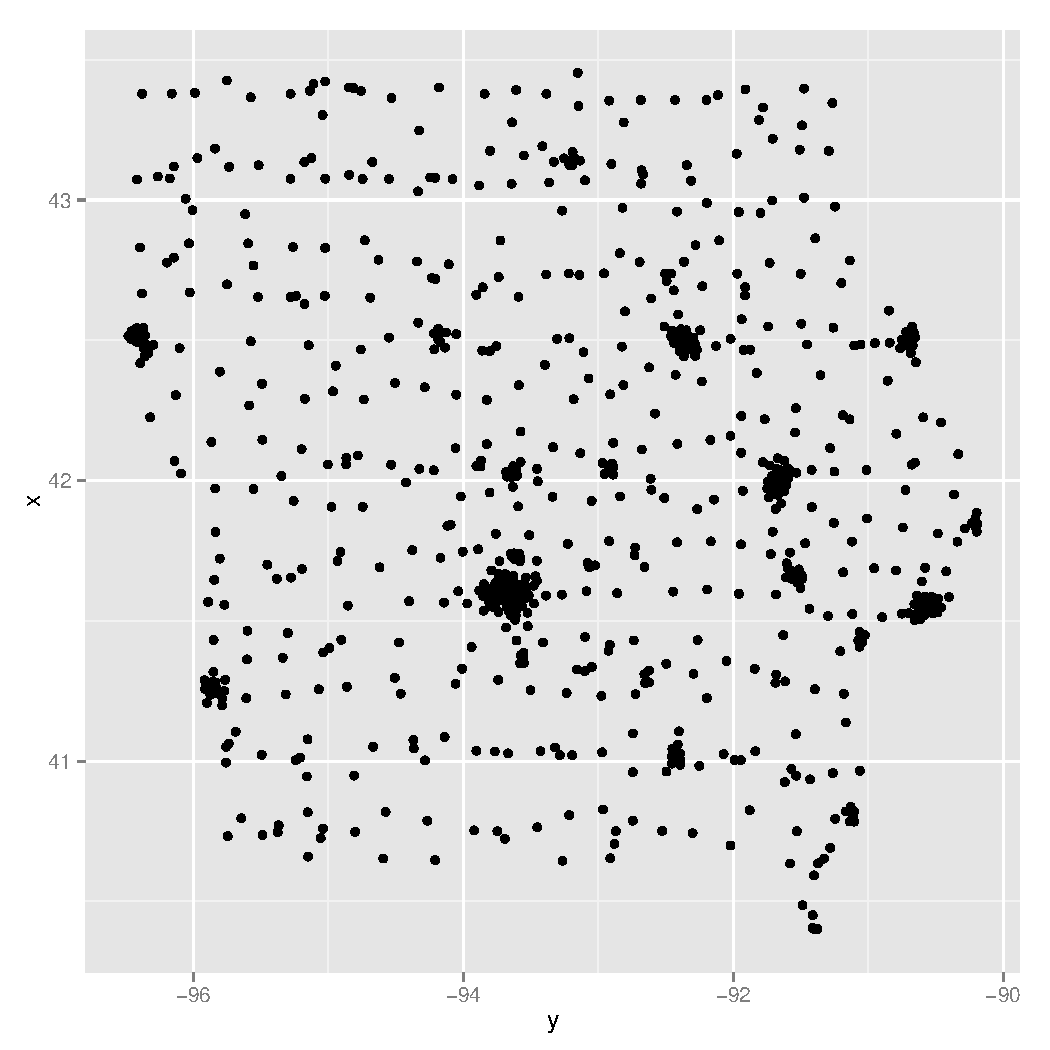
\includegraphics[width=\maxwidth]{figure/minimal-census1} 
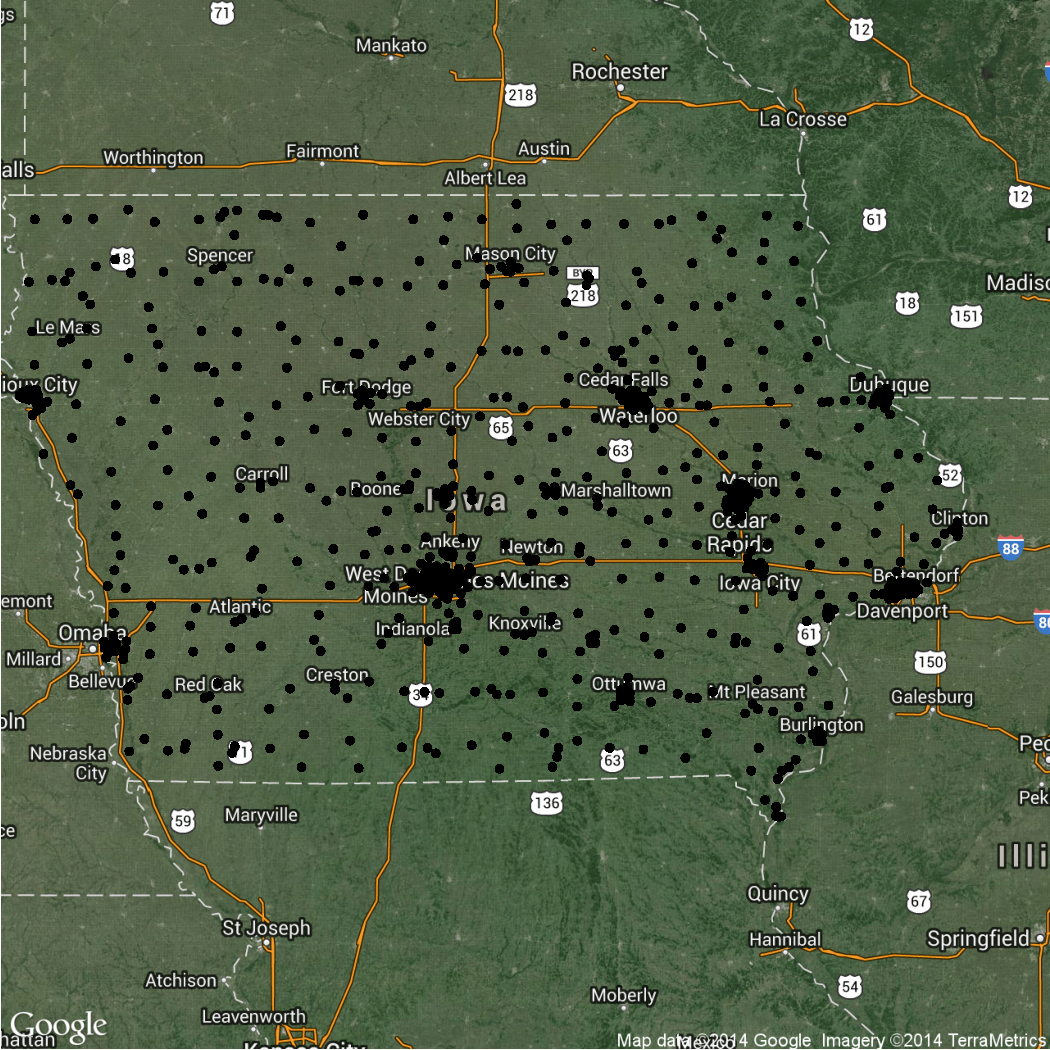
\includegraphics[width=\maxwidth]{figure/minimal-census2} 
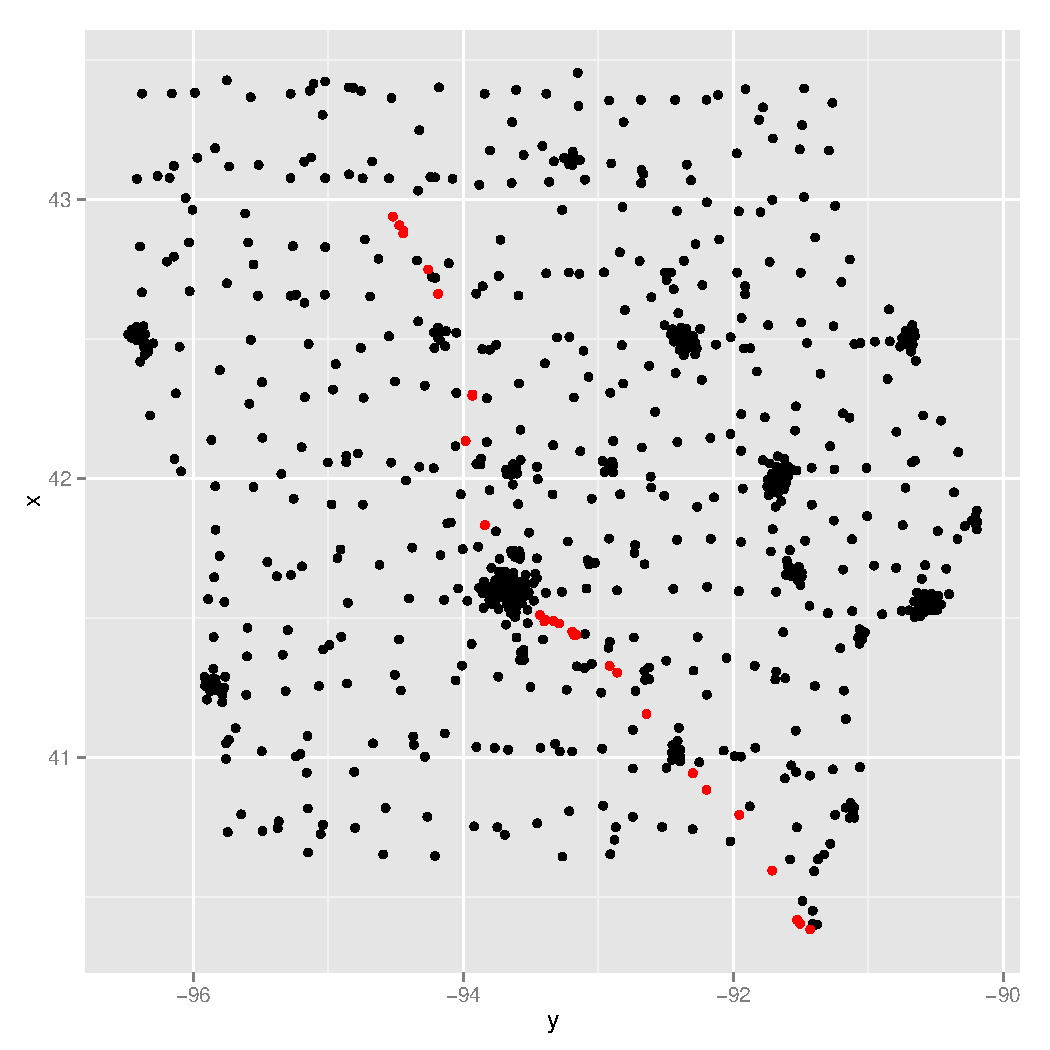
\includegraphics[width=\maxwidth]{figure/minimal-census3} 
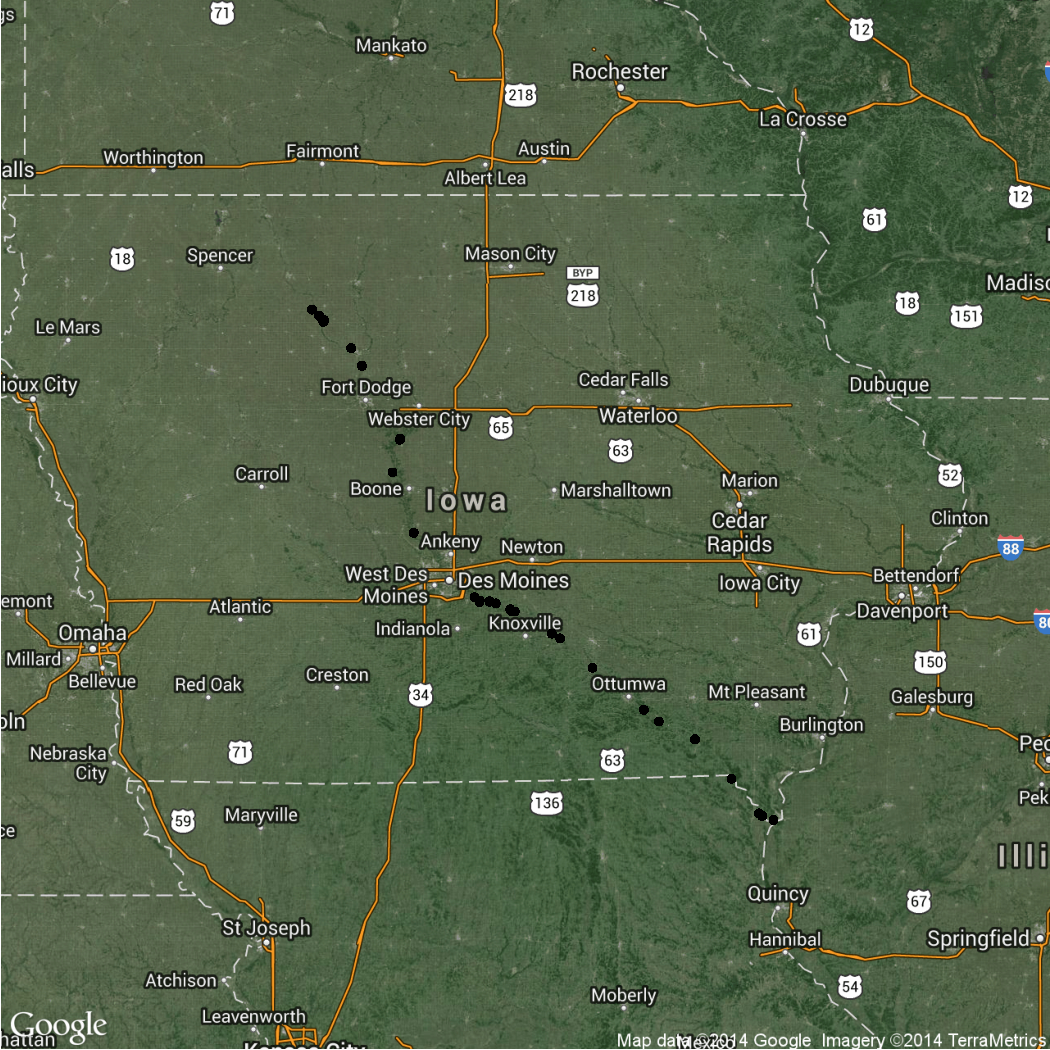
\includegraphics[width=\maxwidth]{figure/minimal-census4} 
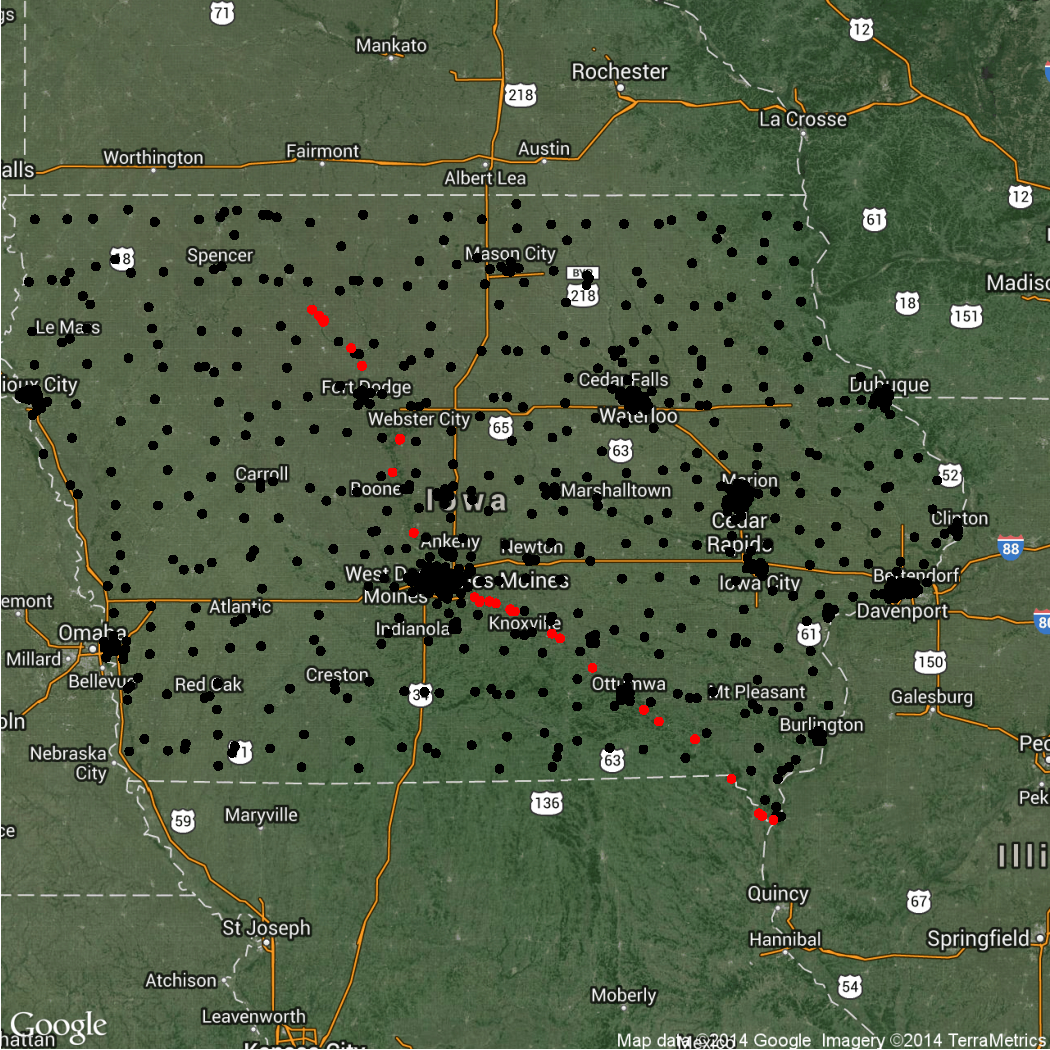
\includegraphics[width=\maxwidth]{figure/minimal-census5} 
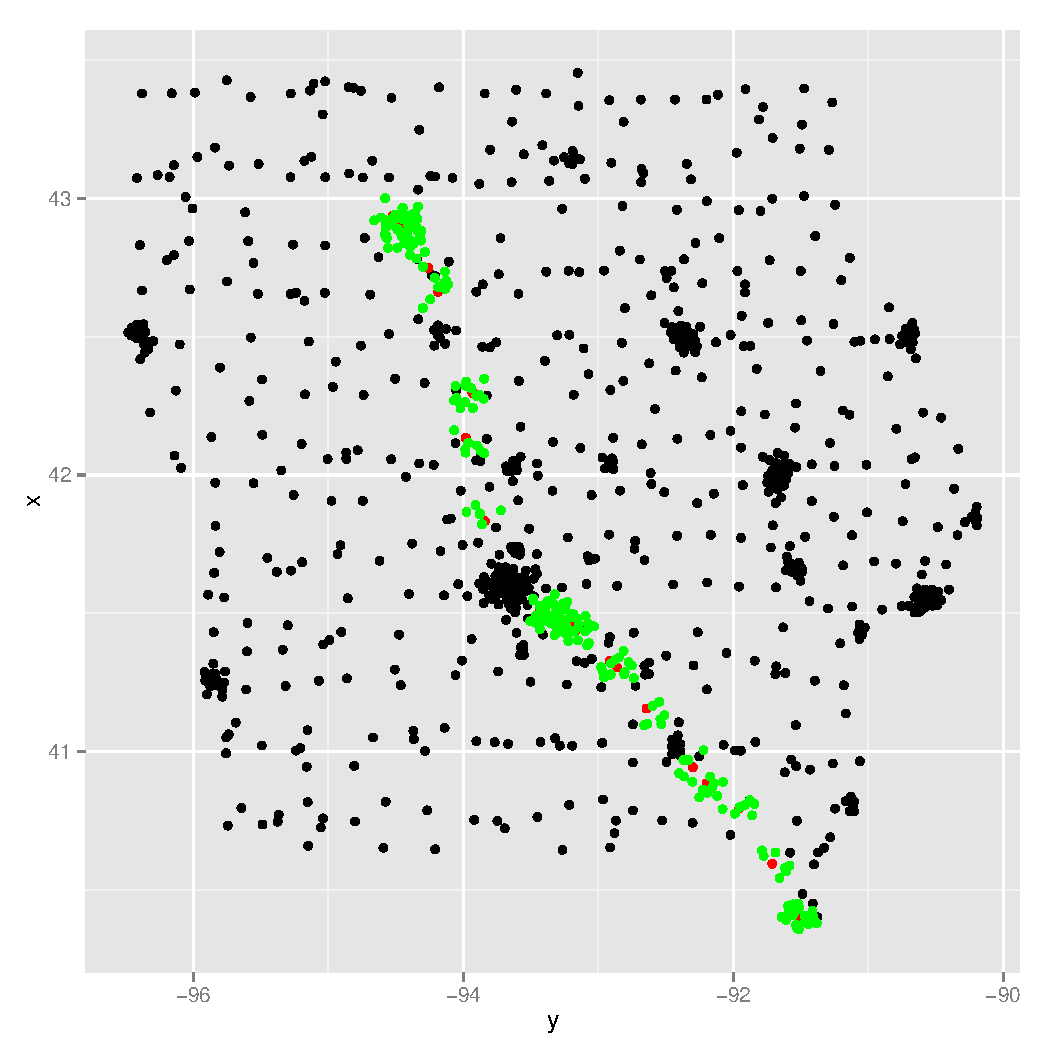
\includegraphics[width=\maxwidth]{figure/minimal-census6} 

}



\end{knitrout}


\section{Results}

We will have to extract the pixel count information available in the CDL data for the points with coordinates in the Census data. By doing this matching, we will construct summaries for all the categories (corn, soybean, etc) for the points in the region of interest. We will do this for the years 2003-2007 and we will report the tables for each year. The final comments would be on the changes in crop categories over this time period and the effect on the future analysis done with the CEAP data. 

\begin{knitrout}
\definecolor{shadecolor}{rgb}{0.969, 0.969, 0.969}\color{fgcolor}\begin{kframe}
\begin{alltt}
\hlcom{# ?cellFromXY cellFromXY}

\hlstd{cdl.pts} \hlkwb{<-} \hlstd{cdl.ia03[}\hlkwd{cellFromXY}\hlstd{(cdl.ia03, loc.newcoords)]}
\end{alltt}


{\ttfamily\noindent\color{warningcolor}{\#\# Warning: some indices are invalid (NA returned)}}\begin{alltt}
\hlkwd{table}\hlstd{(cdl.pts)}\hlopt{/}\hlkwd{length}\hlstd{(cdl.pts[}\hlopt{-}\hlkwd{which}\hlstd{(}\hlkwd{is.na}\hlstd{(cdl.pts))])} \hlopt{*} \hlnum{100}
\end{alltt}
\begin{verbatim}
## cdl.pts
##       1       5      25      28      36      42      44      61      63      82      83 
## 26.6667 30.0000  0.9524  0.4762  4.2857  0.4762  0.4762  5.7143  9.0476  1.4286  3.3333 
##     176 
## 17.1429
\end{verbatim}
\begin{alltt}
\hlstd{cdl.pts} \hlkwb{<-} \hlstd{cdl.ia04[}\hlkwd{cellFromXY}\hlstd{(cdl.ia04, loc.newcoords)]}
\end{alltt}


{\ttfamily\noindent\color{warningcolor}{\#\# Warning: some indices are invalid (NA returned)}}\begin{alltt}
\hlkwd{table}\hlstd{(cdl.pts)}\hlopt{/}\hlkwd{length}\hlstd{(cdl.pts[}\hlopt{-}\hlkwd{which}\hlstd{(}\hlkwd{is.na}\hlstd{(cdl.pts))])} \hlopt{*} \hlnum{100}
\end{alltt}
\begin{verbatim}
## cdl.pts
##       1       5      36      61      63      70      81      82      83      88     176 
## 31.9048 21.9048  1.4286  4.2857 10.0000  0.9524  0.9524  3.3333  3.8095  1.4286 20.0000
\end{verbatim}
\begin{alltt}
\hlstd{cdl.pts} \hlkwb{<-} \hlstd{cdl.ia05[}\hlkwd{cellFromXY}\hlstd{(cdl.ia05, loc.newcoords)]}
\end{alltt}


{\ttfamily\noindent\color{warningcolor}{\#\# Warning: some indices are invalid (NA returned)}}\begin{alltt}
\hlkwd{table}\hlstd{(cdl.pts)}\hlopt{/}\hlkwd{length}\hlstd{(cdl.pts[}\hlopt{-}\hlkwd{which}\hlstd{(}\hlkwd{is.na}\hlstd{(cdl.pts))])} \hlopt{*} \hlnum{100}
\end{alltt}
\begin{verbatim}
## cdl.pts
##       1       5      36      61      63      81      82      83      88     176 
## 24.2857 26.6667  0.9524  2.3810 18.5714  0.4762  3.8095  3.3333  3.8095 15.7143
\end{verbatim}
\begin{alltt}
\hlstd{cdl.pts} \hlkwb{<-} \hlstd{cdl.ia06[}\hlkwd{cellFromXY}\hlstd{(cdl.ia06, loc.newcoords)]}
\end{alltt}


{\ttfamily\noindent\color{warningcolor}{\#\# Warning: some indices are invalid (NA returned)}}\begin{alltt}
\hlkwd{table}\hlstd{(cdl.pts)}\hlopt{/}\hlkwd{length}\hlstd{(cdl.pts[}\hlopt{-}\hlkwd{which}\hlstd{(}\hlkwd{is.na}\hlstd{(cdl.pts))])} \hlopt{*} \hlnum{100}
\end{alltt}
\begin{verbatim}
## cdl.pts
##       1       5      28      36      61     111     121     124     141     142     143 
## 30.4762 20.9524  0.9524  0.4762  1.4286  2.3810  3.8095  0.4762 13.8095  0.4762  0.4762 
##     152     176     190     195 
##  1.4286 19.0476  1.4286  2.3810
\end{verbatim}
\begin{alltt}
\hlstd{cdl.pts} \hlkwb{<-} \hlstd{cdl.ia07[}\hlkwd{cellFromXY}\hlstd{(cdl.ia07, loc.newcoords)]}
\end{alltt}


{\ttfamily\noindent\color{warningcolor}{\#\# Warning: some indices are invalid (NA returned)}}\begin{alltt}
\hlkwd{table}\hlstd{(cdl.pts)}\hlopt{/}\hlkwd{length}\hlstd{(cdl.pts[}\hlopt{-}\hlkwd{which}\hlstd{(}\hlkwd{is.na}\hlstd{(cdl.pts))])} \hlopt{*} \hlnum{100}
\end{alltt}
\begin{verbatim}
## cdl.pts
##       1       5      28      36      87     111     121     124     141     176     190 
## 26.1905 17.6190  0.4762  0.4762  0.4762  2.8571  6.1905  0.4762 16.6667 24.7619  1.9048 
##     195 
##  1.9048
\end{verbatim}
\end{kframe}
\end{knitrout}

\end{document}
